
%(BEGIN_QUESTION)
% Copyright 2015, Tony R. Kuphaldt, released under the Creative Commons Attribution License (v 1.0)
% This means you may do almost anything with this work of mine, so long as you give me proper credit

Denne trefase transformator-koblingen kalles stjerne-zigzag (Wye-Zigzag):

$$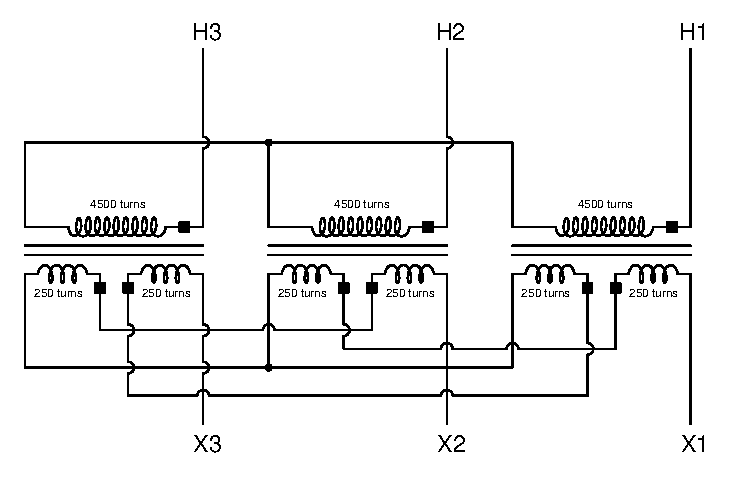
\includegraphics[width=15.5cm]{i00837x01.eps}$$

Beregn beløp og fasevinkel for $V_{X1}$, gitt at $V_{H1}$ er 7.2 kV $\angle$ 0$^{o}$ og at fasefølgen er H1-H2-H3.

\vskip 10pt

$V_{X1}$ = \underbar{\hskip 50pt}

\vfil 

\underbar{file i00837}
\eject
%(END_QUESTION)





%(BEGIN_ANSWER)

Dette er en vurdert oppgave -- ingen svar eller hint oppgis!

%(END_ANSWER)





%(BEGIN_NOTES)

Hvis $V_{H1}$ = 7200 volt $\angle$ 0$^{o}$ og rotasjonen er H1-H2-H3, må primærfasespenningene være:

\begin{itemize}
\item{} $V_{H1}$ = 7200 V $\angle$ $0^{o}$
\item{} $V_{H2}$ = 7200 V $\angle$ $-120^{o}$
\item{} $V_{H3}$ = 7200 V $\angle$ $-240^{o}$
\end{itemize}

Viklingsforholdet 4500:250 (18:1) fra hver primærvikling til hver sekundærvikling gir sekundærviklingsspenninger på 400 volt hver. Da er det nyttig å merke skjemaet med + og $-$ polaritetssymboler (som i en DC-analyse) med kjente spenninger:

$$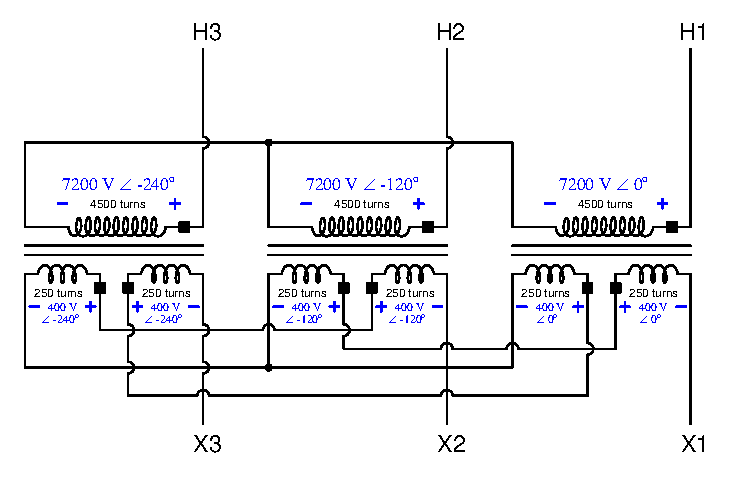
\includegraphics[width=15.5cm]{i00837x02.eps}$$

Merk at alle sekundærviklingsspenningene har samme vinkel som de respektive primærviklingsspenningene, siden vi antar neglisjerbar faseforskyvning i transformatoren. Merk også at alle + og $-$-markeringer følger samme mønster som ``square''-polaritetsmarkeringene på viklingene: hver ``polarity''-terminal er positiv, mens hver ``nonpolarity''-terminal er negativ.

\vskip 10pt

Nå kan vi summere viklingsparspenningene for hver sekundærlinje med riktig polaritet:

\begin{itemize}
\item{} $V_{X1}$ = (400 V $\angle$ $-120^{o}$) $-$ (400 V $\angle$ $0^{o}$) = 692.8 V $\angle$ $-150^{o}$
\item{} $V_{X2}$ = (400 V $\angle$ $-240^{o}$) $-$ (400 V $\angle$ $-120^{o}$) = 692.8 V $\angle$ $90^o$
\item{} $V_{X3}$ = (400 V $\angle$ $0^{o}$) $-$ (400 V $\angle$ $-240^{o}$) = 692.8 V $\angle$ $-30^o$
\end{itemize}

\filbreak

Fasordiagrammet for sekundærviklingsspenningene viser tydelig hvorfor dette kalles ``zigzag''-kobling. Pilspissene på viklingsfasorene viser subtraksjonen, med fasorspisser som møtes i hvert hjørne av ``zigzag''-formen:

$$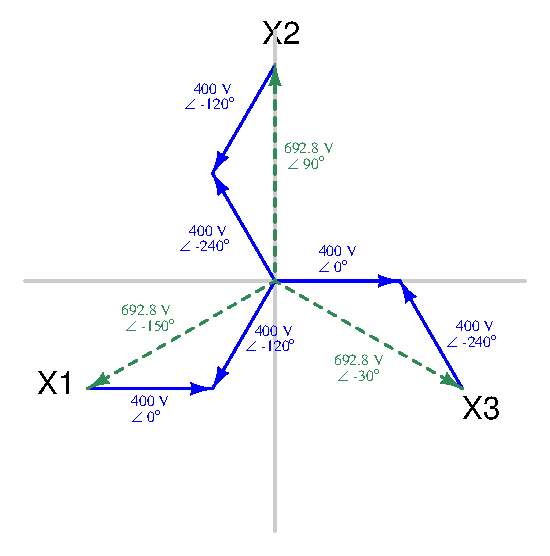
\includegraphics[width=15.5cm]{i00837x03.eps}$$

Resultantfasorene $V_{X1}$, $V_{X2}$ og $V_{X3}$ er vist i grønt, mens sekundærviklingsfasorene er vist i blått.

%INDEX% Electronics review, 3-phase transformer bank phase shift calculations

%(END_NOTES)
